\documentclass[tikz,border=2pt,11pt]{standalone}
\usetikzlibrary{arrows.meta}
\usepackage{amsmath}
\usepackage{amssymb}
\usepackage{tikz}
\newcommand{\Z}{\mathbb Z}
\newcommand{\Q}{\mathbb Q}
\newcommand{\C}{\mathbb C}
\newcommand{\R}{\mathbb R}
\newcommand{\N}{\mathbb N}
\newcommand{\HH}{\mathcal H}
\newcommand{\KK}{\operatorname{KK}}
\newcommand{\SL}{\operatorname{SL}}
\newcommand{\tr}{\operatorname{tr}}
\newcommand{\prop}{\operatorname{prop}}
\newcommand{\Ad}{\operatorname{Ad}}
\newcommand{\supp}{\operatorname{supp}}
\newcommand{\lf}{\mathrm{lf}}
\newcommand{\id}{\mathrm{id}}
\newcommand{\abs}[1]{\lvert #1\rvert}
\newcommand{\norm}[1]{\lVert #1\rVert}
\begin{document}
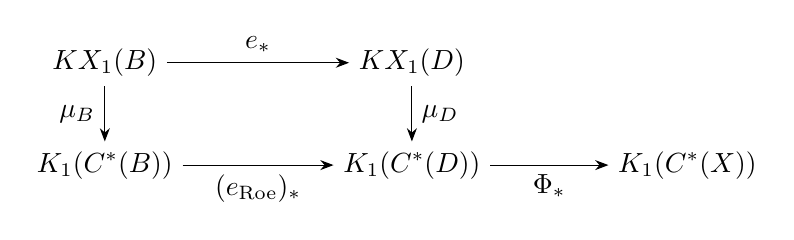
\begin{tikzpicture}[baseline=(current bounding box.center),>=Stealth]
 \node (a) at (0,1.3) {$KX_1(B)$};
 \node (b) at (3.9,1.3) {$KX_1(D)$};
 \node (c) at (0,0) {$K_1(C^*(B))$};
 \node (d) at (3.9,0) {$K_1(C^*(D))$};
 \node (f) at (7.4,0) {$K_1(C^*(X))$};
 \draw[->] (a)--node[above]{$e_*$}(b);
 \draw[->] (a)--node[left]{$\mu_B$}(c);
 \draw[->] (b)--node[right]{$\mu_D$}(d);
 \draw[->] (c)--node[below]{$(e_{\mathrm{Roe}})_*$}(d);
 \draw[->] (d)--node[below]{$\Phi_*$}(f);
\end{tikzpicture}
\end{document}
